\section{Tuning}\label{sec:tuning}

\textbf{Search.} Optuna \citep{akiba2019optuna} ran \TuneTrials{} trials of its tree-structured Parzen estimator
(seed 42), each scored as the mean development wMAE over the five folds. The locked test was never used. The search
covered the ridge penalty (0.001--10), spline knots (distance 5--12, coordinates 4--9, weight 4--7), the tree
stage (50--600 trees, learning rate 0.01--0.15, 7--63 leaves, 20--300 loads per leaf, L2 penalty 0.001--30,
50--100\% of columns per tree) and recency weighting (off, or a time constant of 45--720 days).

\textbf{Result.} The best trial scores \usd{\TuneBest}; the untuned model scores \usd{\DevStepE}. The best trial is
the configuration frozen in \texttt{configs/final.yaml} (re-found: \TuneMatchesFinal). Table~\ref{tab:tuned} lists
it. The tree stage's size and learning rate matter most (Table~\ref{tab:importance}).

\begin{table}[H]
  \centering
  \begin{minipage}[t]{0.55\linewidth}\centering
    \captionof{table}{Tuned settings.}\label{tab:tuned}
    \small\begin{tabular}{lr}
\toprule
Setting & Tuned value \\
\midrule
Ridge penalty alpha & 0.265 \\
Spline knots: distance / weight / coordinates & 5 / 7 / 4 \\
Recency time constant (days) & 122.6 \\
Residual trees & 293 \\
Learning rate & 0.0215 \\
Leaves per tree & 62 \\
Minimum loads per leaf & 90 \\
L2 penalty lambda & 3.26 \\
Share of columns per tree & 0.81 \\
\bottomrule
\end{tabular}

  \end{minipage}\hfill
  \begin{minipage}[t]{0.4\linewidth}\centering
    \captionof{table}{Most important settings.}\label{tab:importance}
    \small\begin{tabular}{lr}
\toprule
Hyperparameter & Importance (fANOVA) \\
\midrule
n estimators & 0.43 \\
dist knots & 0.12 \\
reg lambda & 0.09 \\
learning rate & 0.09 \\
min child samples & 0.08 \\
\bottomrule
\end{tabular}

  \end{minipage}
\end{table}

\begin{figure}[H]
  \centering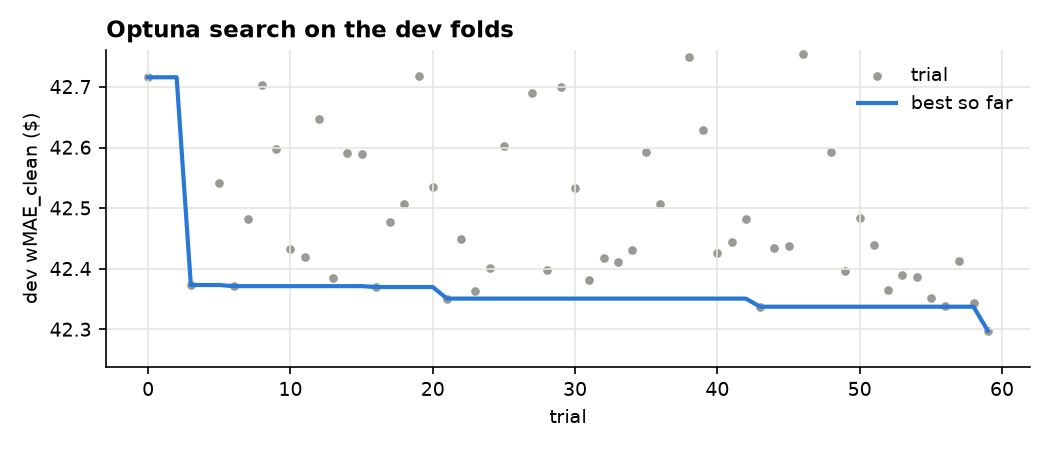
\includegraphics[width=0.75\linewidth]{tuning.png}
  \caption{Trial scores and the best score so far.}
\end{figure}

\textbf{Is the gain real?} Tuning and scoring on the same folds flatters the tuned model. To check, we re-tuned on
folds 1 to $k-1$ only and scored fold $k$ (Table~\ref{tab:nested}). The gains on these unseen folds,
\usd{\NestedGainFour} and \usd{\NestedGainFive}, are close to the in-sample gain of \usd{\DevTunedGain}.

\begin{table}[H]
  \caption{Forward-nested check: tune on earlier folds, score the next one.}\label{tab:nested}
  \inputtable{nested}
\end{table}

\textbf{Honest note.} On the locked test the untuned model was slightly better (Section~\ref{sec:evaluation}). Tuned
and default settings differ by about \TunedDefaultTestPct\% on the test, and by similar amounts in the other
direction on the development folds. They are practically
equivalent. We kept the tuned model because the selection rule was fixed before the test was opened.
